\documentclass[10pt]{article}
\usepackage{graphicx}
\usepackage{subcaption}
\usepackage[T1]{fontenc}
\usepackage{amsmath}
\usepackage{lipsum}
\usepackage{amsfonts}
\usepackage{hyperref}
\usepackage[utf8]{inputenc}
\usepackage[letterpaper,margin=1in]{geometry}
\usepackage[parfill]{parskip}
\usepackage[europeanresistors, american]{circuitikz}
\usetikzlibrary{arrows,shapes,calc,positioning}
\usetikzlibrary{shapes}
\usetikzlibrary{plotmarks}
\usepackage{tikz}
\usepackage{pgfplots}
\usepackage{xparse}
\usetikzlibrary{decorations.markings,positioning}
\definecolor{whitesmoke}{rgb}{0.90, 0.90, 0.90}
\definecolor{lightgray}{rgb}{0.73, 0.73, 0.73}% overrides default?
\definecolor{dimgray}{rgb}{0.51, 0.51, 0.51}
\pgfplotsset{compat=newest}
\usepgfplotslibrary{units}
\newcommand{\oscope}[2] % #1 = name , #2 = rotation angle
{
    \draw[thick,rotate=#2] (#1) circle (12pt)
    (#1) ++(-0.35,-0.1) -- ++(0.3,0.3) --++(0,-0.3)-- ++(0.3,0.3) --++(0,-0.3);
}
\def\therefore{\boldsymbol{\text{ }
\leavevmode
\lower0.4ex\hbox{$\cdot$}
\kern-.5em\raise0.7ex\hbox{$\cdot$}
\kern-0.55em\lower0.4ex\hbox{$\cdot$}
\thinspace\text{ }}}

\vspace{-8ex}
\date{}
\begin{document}

\title{\textbf{\Large{\textsc{ECE320:} Fields and Waves}} \\ \Large{Lab 3 Report: Design of a Double Stub Matching Network} \\ \textbf{\small{PRA106}}\vspace{-0.3cm}}
\author{Alp Tarım, Pranshu Malik \\ \footnotesize{1003860128}, \footnotesize{1004138916}}

\maketitle

\section{Introduction}

This laboratory session was focused on investigating the input impedance and reflection coefficient at the load, and
making transformations to the load impedance using a double stub network such that we are able to match the input impedance 
to the transmission line. We also measured the voltage standing wave ratio (VSWR) for the same matching network to characterize
its bandwidth. Figure 1 shows the schematic for a double-stub tuner and its equivalent circuit. Our theoretical work 
and measurements are based on the unknown \underline{"orange"} labelled load given to us. 

\begin{figure}[h]
  \centering
  \begin{circuitikz}
    \draw
    (0,2) to [esource, l_=$\text{VNA}$] (0, 0) -- (2,0)
    to [tline, o-o] (4,0)
    to [tline, *-o] (6,0)
    to [tline, o-*] (8,0) -- (8.5,0)
    to [R, l_=$Z_L$] (8.5, 2) -- (8,2)
    to [tline, l=${d_0}$,*-o] (6,2)
    to [tline, o-o, l=${d_1}$] (4,2)
    to [tline, l=${Z_0, \beta, L}$, *-o] (2,2)
    to [R, l_=${Z_\text{VNA}=Z_0}$] (0, 2);

    \draw[thick] (6,2) -- (7, 0.5) -- (7,-1.5) -- (6,0);
    \draw[thick] (4,2) -- (5, 0.5) -- (5, -1.5) -- (4,0);
    \draw (0,0) to[short, *-*] node[ground]{} (0,0);
    \draw (6.2, -0.75) node{$L_1$} (6.2, -0.75);
    \draw (4.2, -0.75) node{$L_2$} (4.2, -0.75);
    \draw (5.75, 1) node{$Z_0, \beta$} (5.75, 1);
    \draw [dotted, thick] (4,-0.35) -- (4,2.35) (8,-0.35) -- (8,2.35);


    \draw
    (0,-2) to [esource, l_=$\text{VNA}$] (0, -4) -- (2,-4)
    to [tline, o-o] (4,-4)
    to [tline, *-o] (6,-4)
    to [tline, o-*] (8,-4) -- (8.5,-4)
    to [R, l_=$Z_L$] (8.5, -2) -- (8,-2)
    to [tline, l=${d_0}$,*-o] (6,-2)
    to [tline, o-o, l=${d_1}$] (4,-2)
    to [tline, l=${Z_0, \beta, L}$, *-o] (2,-2)
    to [R, l_=${Z_\text{VNA}=Z_0}$] (0, -2);

    \draw (0,-4) to[short, *-*] node[ground]{} (0,-4);
    \draw (4,-4) to [R, l=$jb_2$] (4,-2);
    \draw (6,-4) to [R, l=$jb_1$] (6,-2);
  \end{circuitikz}
  \caption{A double-stub matching network}
\end{figure}


\section{Measurement of the Unknown Load Impedance}

We measured load impedance on a Smith Chart using the VNA, shown in Figure 2 (a). The values of the 
(de-embedded) load impedance with its normalized form taking $Z_0=50\Omega$ are: 

\begin{align*}
  Z_L &= 31.08 + 9.32j \quad [\Omega]\\
  Z_\text{L,N} &= 0.622 + 0.186j\\
  Y_\text{L,N} &= 1.476 - 0.441j
\end{align*}

Also, if we rotate $Z_\text{L,N}$ by $0.16\lambda$, we end up very near $Y_A$ giving us $Z_\text{L,N}' = 0.85 - 0.45j$ 
corresponding to $Z_L' = 42.5 - 22.5j [\Omega]$ which closely matches the result shown by the VNA in Figure x. 

\begin{figure}[ht]
  \centering
  \begin{subfigure}[b]{0.45\textwidth}
      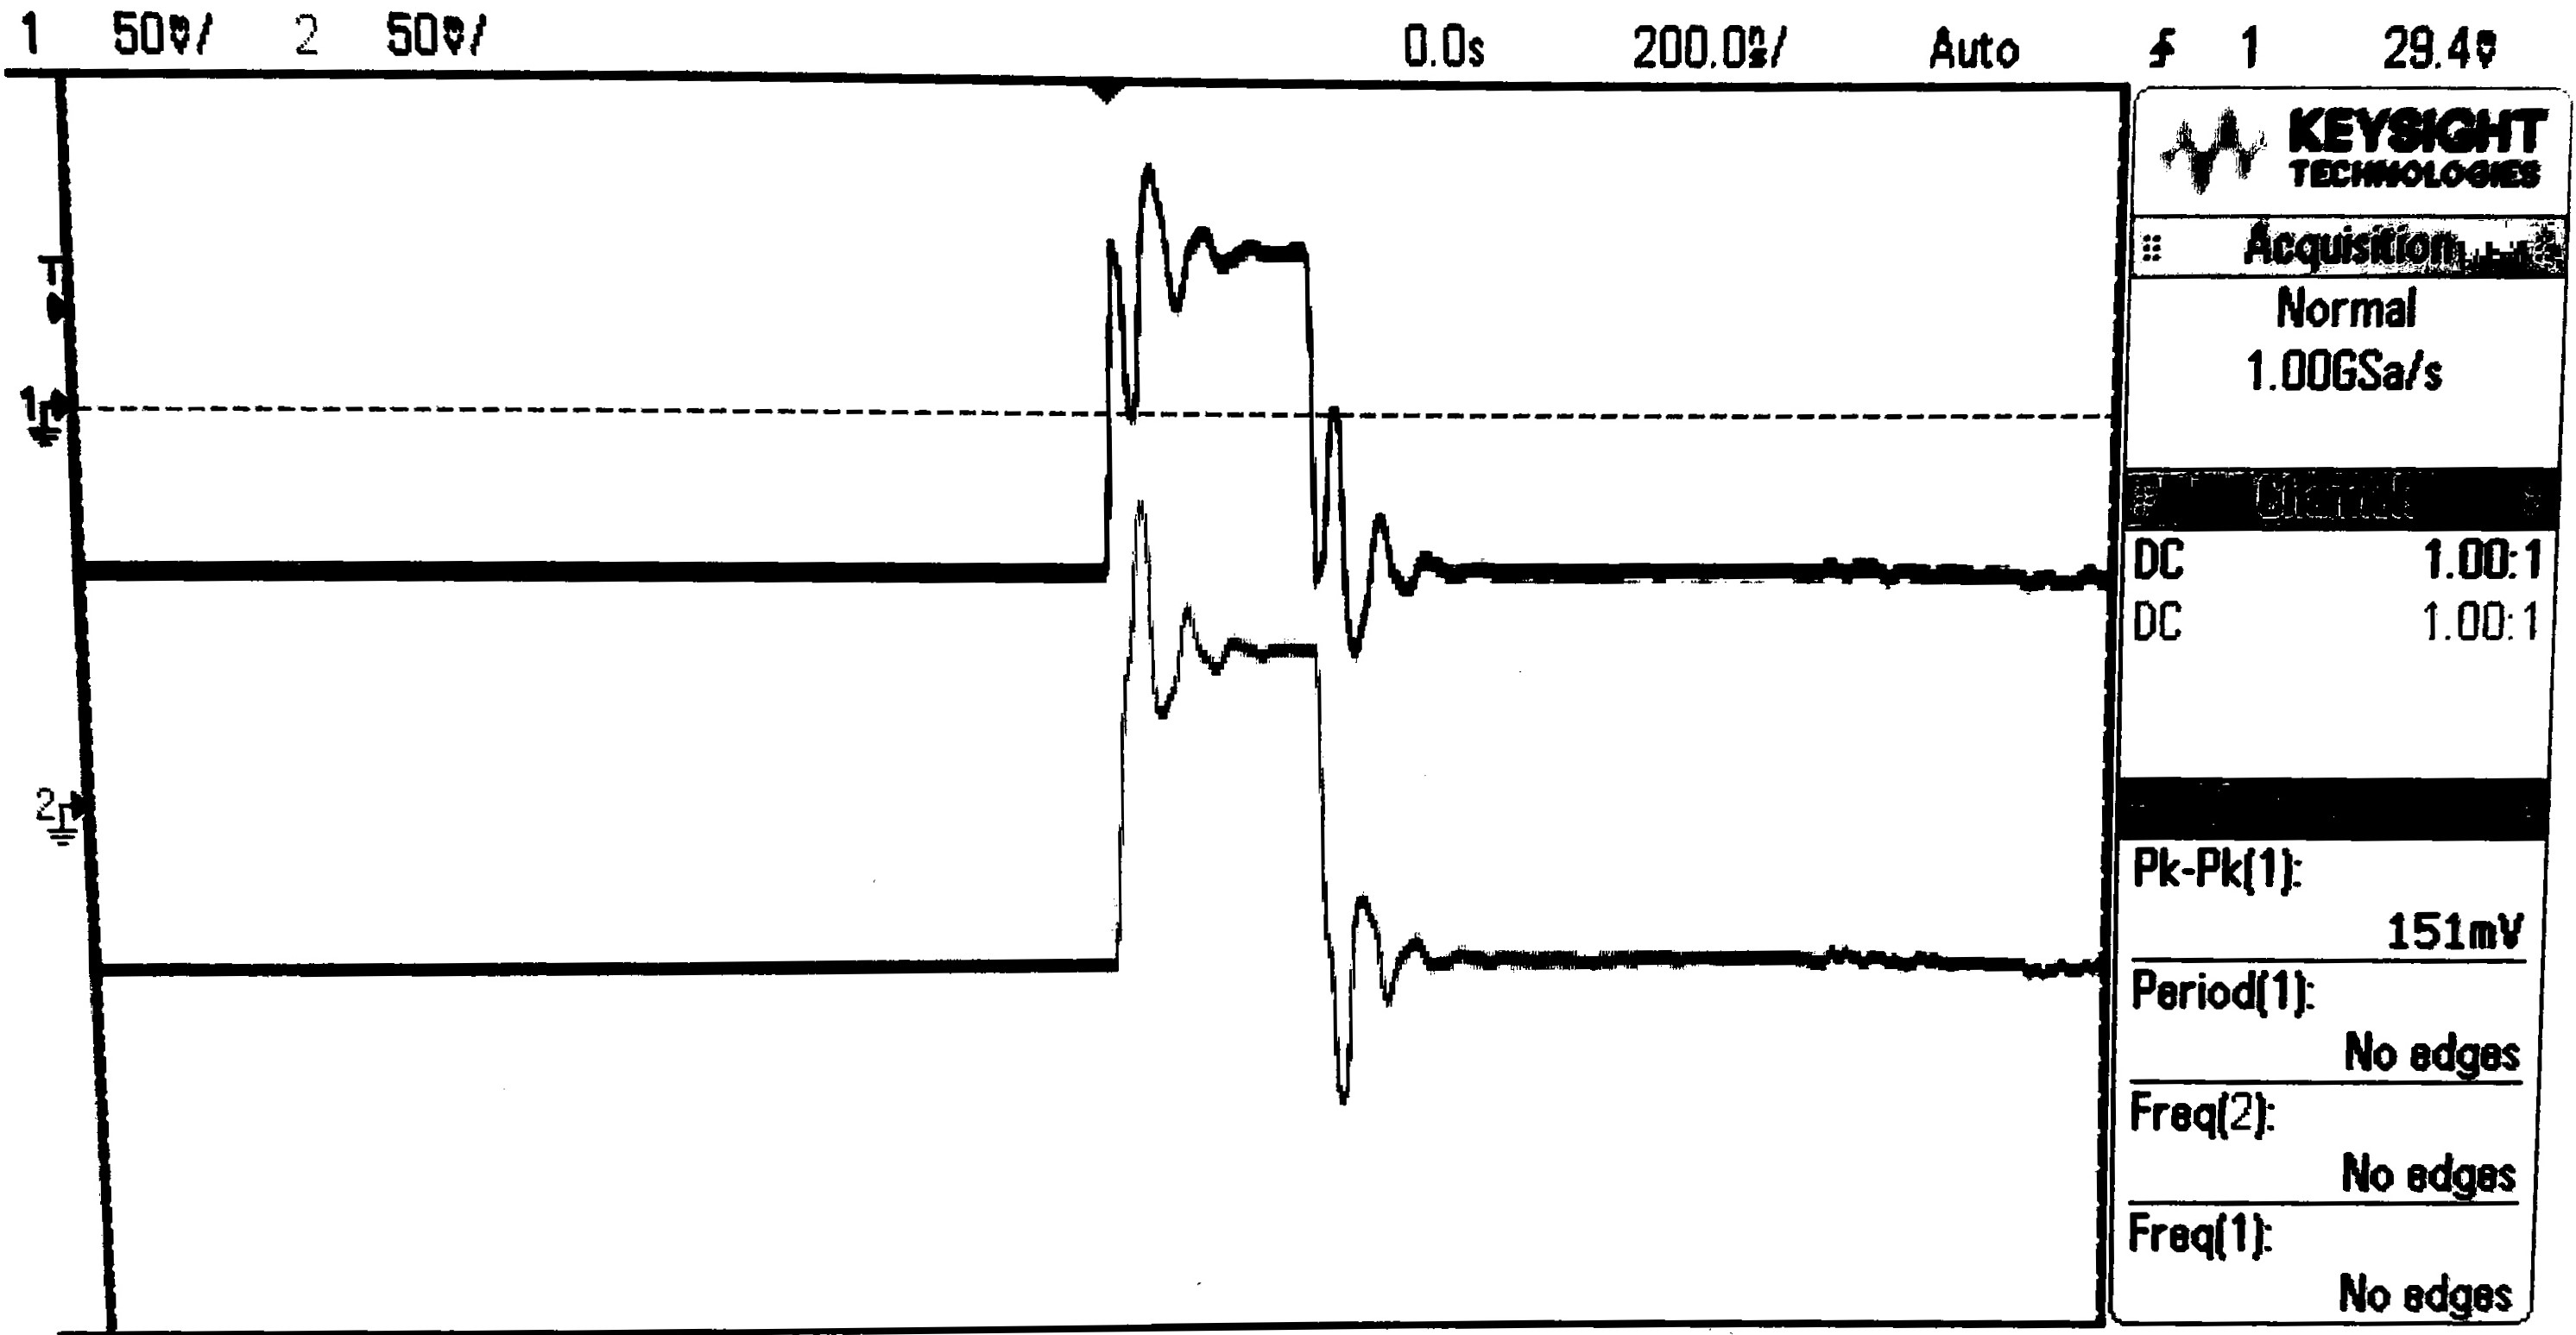
\includegraphics[width=\textwidth]{../photos/lab1/v_t_pt_c.jpg}
      \caption{Port C $(0\text{m})$}
  \end{subfigure}
  \quad
  \begin{subfigure}[b]{0.45\textwidth}
      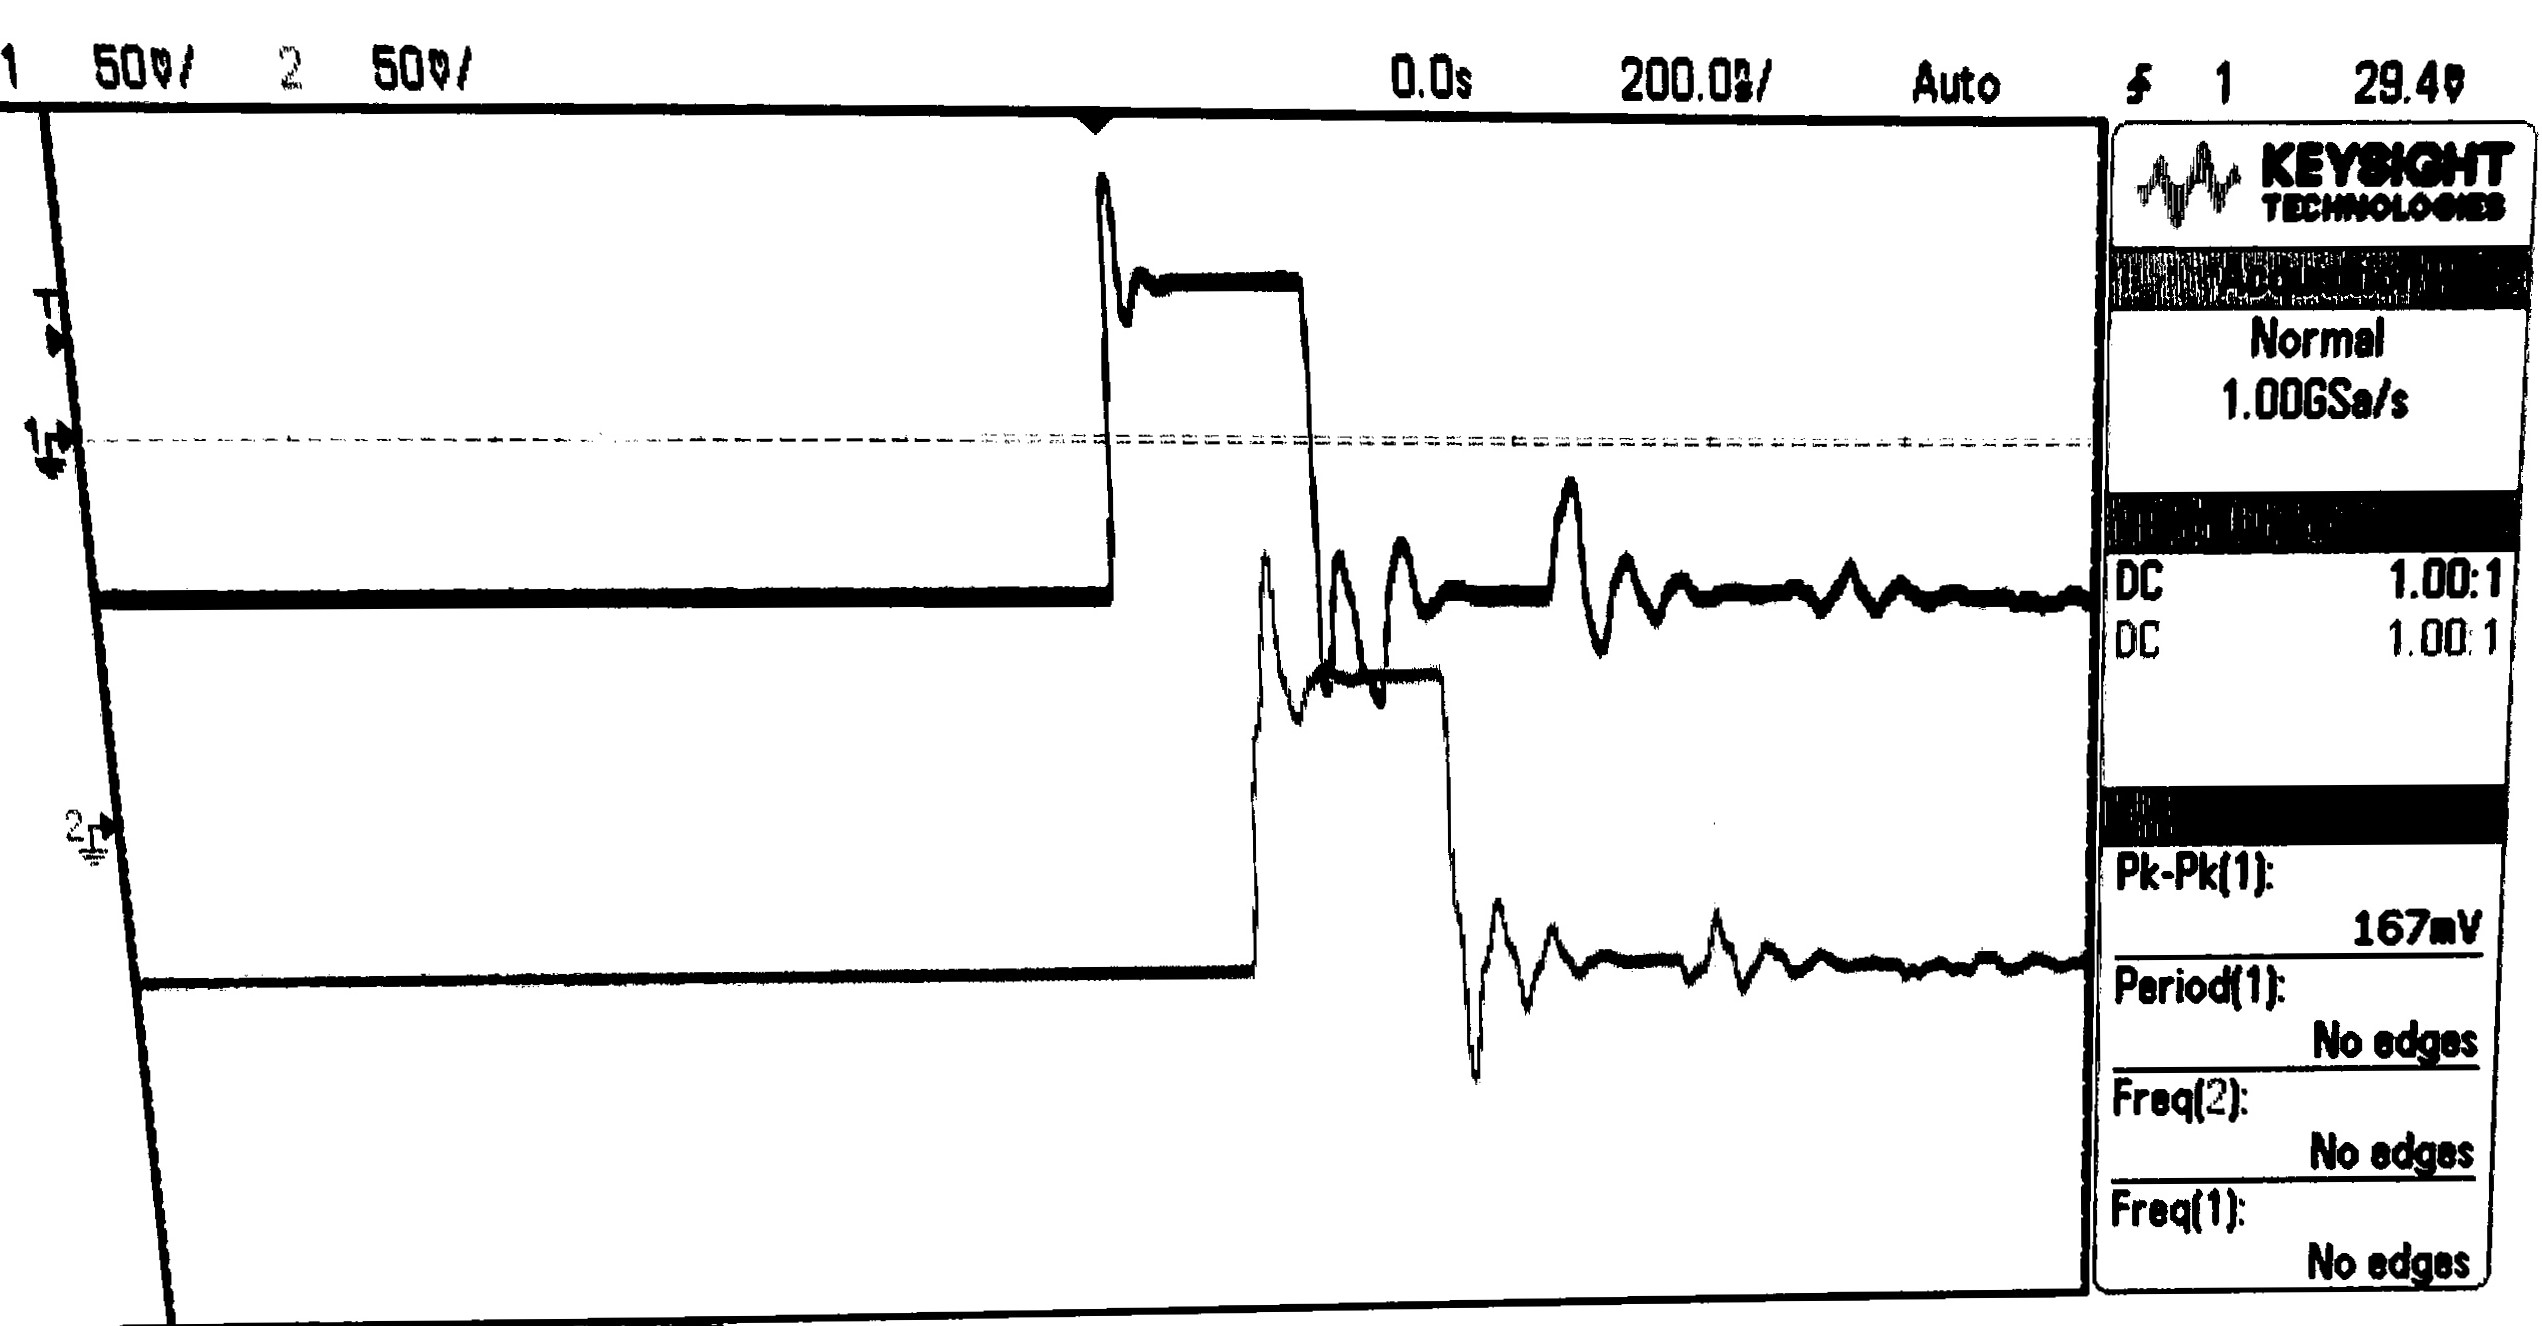
\includegraphics[width=\textwidth]{../photos/lab1/v_t_pt_d.jpg}
      \caption{Port D $(30\text{m})$}
  \end{subfigure}
  \caption{Measured $V(t)$ at different loactions along the transmission line with $Z_L = Z_0$ \vspace{-0.5cm}}
  \label{v_t_matched_tline}
\end{figure}

\section{Smith Charts and the Graphical Matching Process}

We are asked to do a double stub matching. However, it requires some extra steps compared to single stub matching
including the rotation of the unit circle and movement of vertain values along with it. Addition of the second stub
causes this complication as explained in the lab document. The smith chart and our calculations for the lengths of 
our stubs are attached.

\section{Designing a Double-stub Matching Network}
\begin{table}
  \[
      \begin{array}{c|c}
          \textbf{Parameter} & \textbf{Value} \\ \hline
          L_1 & 12.15 \text{ cm}\\
          L_2 & 7.88 \text{ cm}\\
          L_1' & 16.88 \text{ cm}\\
          L_2' & 16.69 \text{ cm}
      \end{array}
  \]
  \caption{Theoretically calculated stub length pairs}
\end{table}

\section{Experimental Determination }
\begin{table}
  \[
      \begin{array}{c|c}
          \textbf{Parameter} & \textbf{Value} \\ \hline
          L_1 & 1232 \text{ cm}\\
          L_2 & 1232 \text{ cm}\\
          L_1' & 1232 \text{ cm}\\
          L_2' & 1232 \text{ cm}
      \end{array}
  \]
  \caption{Experimentally measured stub lengths}
\end{table}
\section{Bandwidth Calculations}

a)  Bandwidth smaller than 2
    The y-axis is VSWR and VSWR=(1+gamma)/(1-gamma). For this value to be less than or equal to 2, gamma has to be
    less than or equal to 0.33. 
b)  Bandwidth limitation
    In terms of the bandwidth, shorter lines perform better. Longer lines change impedance faster compared
    to shorter lines when the frequency is modified. The reason for that is the following:
    Consider a lossless line, alpha is zero in this case and we only have j beta. This expression is also 
    equal to w*sqrt(LC)*j. So w*sqrt(LC)=beta. Now, Zin = Z0(Zl+jZ0tan(beta*l)/(Z0+jZltan(beta*l))) and
    reflection coef.= (Zl-Z0)/(Zl+Z0). When l in the first equation is large then a small change in beta (meaning in w)
    is going to result in a large change in Zin because of tan(beta*l) function. Consequently a large jump in reflection coefficient. 
    Since reflection coefficient has to be less than 0.33 there is a smaller window of frequencies we can use
    and fit in this constraint. However, when l is smaller (ie. shorter line) we can modify w much more and
    still stay in the necessary bound of values for the reflection coefficient. 
    For 20log(|gamma|) when gamma=1/3 20log(|gamma|)~-10dB. This suggests magnitudes smaller than -10 dB are 
    acceptable values for gamma (so that the reflection doesn't modify the final value as much).
c)  Measurements
    Our measurements were pretty close within an error of 2 cm. Considering the number of operations we did
    on the smith chart with pencil and paper, we received accurate values. Additionally measurements on 
    the double stub matching network are also susceptible to error.

\section{Notes}

All images taken during the lab were post-processed in a batch using a custom script
that bit-wise inverts the pixels and binarizes the resulting image based on a custom threshold.
No adjustments or modifications were made to the readings, for which the measurements on the VNA
are also shown alongside the waveforms. All scripts and related work can be found at 
\href{https://github.com/pranshumalik14/ece320-labs}{\texttt{github.com/pranshumalik14/ece320-labs}}.

\end{document}